% -*- TeX -*- -*- UK -*- -*- Soft -*-


\part{Evolutionary Algorithms}

\chapter{Evolutionary Algorithms Overview}
\label{chap:EvolAlgoOverview}


\section{Introduction}

``In artificial intelligence, an \ac{EAlg} is a subset of evolutionary computation, a generic population-based metaheuristic optimization algorithm. An EA uses mechanisms inspired by biological evolution, such as reproduction, mutation, recombination, and selection. Candidate solutions to the optimization problem play the role of individuals in a population, and the fitness function determines the quality of the solutions. Evolution of the population then takes place after the repeated application of the above operators.

``Evolutionary algorithms often perform well approximating solutions to all types of problems because they ideally do not make any assumption about the underlying fitness landscape.  In most real applications of EAs, computational complexity is a prohibiting factor. In fact, this computational complexity is due to fitness function evaluation. Fitness approximation is one of the solutions to overcome this difficulty. However, seemingly simple EA can solve often complex problems; therefore, there may be no direct link between algorithm complexity and problem complexity.''\cite{WikipeadiaEvolutionaryAlgo2019}

Genetic Algorithm was developed by John Holland in 1975. It was shown that it can be used to solve an optimization problem by his student Goldberg, who used genetic algorithms to control gas pipeline transmission. Since then, genetic algorithms have remained popular, and have inspired various other evolutionary programs \cite{Mathur2019}.


Genetic algorithms offer some intriguing advantages and can produce results when the tradition gradient-based approaches fail \cite{Mathur2019}:

Advantages:
\begin{enumerate}
\item They can be used to optimize either continuous or discrete variables.

\item Unlike gradient descent, we do not require derivative information, which also means that there is no need for the fitness function to be continuous and differentiable.

\item It can simultaneously search from a wide sampling of the cost surface.

\item We can deal with a large number of variables without a significant increase in computation time.

\item The generation of the population and calculating their fitness values can be performed in parallel, and hence genetic algorithms are well suited for parallel computers.

\item They can work even when the topological surface is extremely complex because crossover and mutation operators help them in jumping out of a local minimum.

\item They can provide more than one optimum solution.

\item We can use them with numerically generated data, experimental data, or even analytical functions. They specifically work well for large-scale optimization problems.
\end{enumerate}

Despite the previously mentioned advantages, we still do not find genetic algorithms to be a ubiquitous solution to all optimization problems\cite{Mathur2019}: 
\begin{enumerate}
\item If the optimization function is a well-behaved convex function, then gradient-based methods will give a faster convergence

\item The large population of solutions that helps genetic algorithms cover the search space more extensively also results in slow convergence

\item Designing a fitness function can be a daunting task
\end{enumerate}

\section{Overview: Biological }
\TBC{TBC}

\section{Overview: EA Computation}

The information in this section is taken from \cite{DevinSoni2018,skymind2019,Song2016}.


Genes are Basic instructions for building an organism. Genes are located in chromosomes as sequential form, where each gene represents a specific trait of the organism.

The search space contains \lstinline{Populations} that are collections of \lstinline{Individuals} (the equivalent of a biological chromosome).  Each individual (chromosome) is composed of genes, with each gene describing some trait or property.



Genetic and evolutionary algorithms approach mathematical optimization (how do I maximize or minimize a certain value?) in similar ways. What they have in common are ideas drawn from biology: natural selection, reproduction and genetic mutation.

Evolutionary algorithms are a heuristic-based approach to solving problems that cannot be easily solved in polynomial time, such as classically NP-Hard problems, and anything else that would take far too long to exhaustively process. When used on their own, they are typically applied to combinatorial problems; however, genetic algorithms are often used in tandem with other methods, acting as a quick way to find a somewhat optimal starting place for another algorithm to work off of.

The premise of an evolutionary algorithm (to be further known as an EA) is quite simple given that you are familiar with the process of natural selection. An EA contains four overall steps: initialization, selection, genetic operators, and termination. These steps each correspond, roughly, to a particular facet of natural selection, and provide easy ways to modularize implementations of this algorithm category. Simply put, in an EA, fitter members will survive and proliferate, while unfit members will die off and not contribute to the gene pool of further generations, much like in natural selection.

\begin{marginfigure}
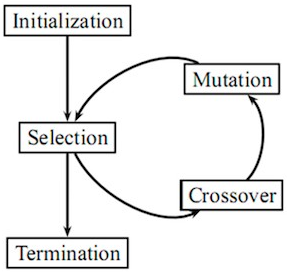
\includegraphics{GA-overview}
\end{marginfigure}

We generally define the problem as such: we wish to find the best combination of elements that maximizes some fitness function, and we will accept a final solution once we have either ran the algorithm for some maximum number of iterations, or we have reached some fitness threshold. This scenario is clearly not the only way to use an EA, but it does encompass many common applications in the discrete case

The process generally plays out as follows:

\begin{enumerate}
\item Randomly initialize population(t)

\item Evaluate fitness of population(t)

\item Repeat
\begin{enumerate}
\item Select parents from population(t)

\item Perform crossover on parents creating population(t+1)

\item  Perform Mutation of population(t+1)

\item Evaluate fitness of population(t+1)
\end{enumerate}
\item Until best individual is good enough
\end{enumerate}


\subsection{Initialization}
In order to begin our algorithm, we must first create an initial population of solutions. The population will contain an arbitrary number of possible solutions to the problem, oftentimes called members. It will often be created randomly (within the constraints of the problem) or, if some prior knowledge of the task is known, roughly centered around what is believed to be ideal. It is important that the population encompasses a wide range of solutions, because it essentially represents a gene pool; ergo, if we wish to explore many different possibilities over the course of the algorithm, we should aim to have many different genes present.

\subsection{Selection}
Once a population is created, members of the population must now be evaluated according to a fitness function. A fitness function is a function that takes in the characteristics of a member, and outputs a numerical representation of how viable (goodness) of a solution it is in terms of the problem. Creating the fitness function can often be very difficult, and it is important to find a good function that accurately represents the data; it is very problem-specific. Fitness may be determined by an objective function or by
subjective judgement. The model calculates the fitness of all members, and selects a portion of the top-scoring members, allowing them to pass on their properties or genes to the next generation.

The process of natural selection kills living beings that are unfit for their environments, while those more suited to that environment, by definition, survive and reproduce more prolifically. Thus, those individuals who survived long enough to breed successfully were “selected” by nature, which imposes a rough filter of predators and toxins on the organisms within it, and cuts many threads short. The value these individuals are maximizing is their number of descendents, or copies of their genes circulating in the gene pool.



\subsection{Multiple objective functions}

EAs can also be extended to use multiple fitness functions. This complicates the process somewhat, because instead of being able to identify a single optimal point, we instead end up with a set of optimal points when using multiple fitness functions. The set of optimal solutions is called the Pareto frontier, and contains elements that are equally optimal in the sense that no solution dominates any other solution in the frontier. A decider is then used to narrow the set down a single solution, based on the context of the problem or some other metric.


\begin{marginfigure}
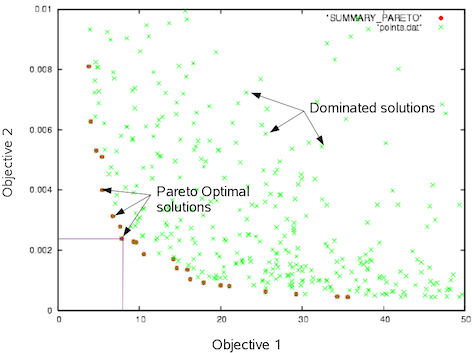
\includegraphics{GA-pareto-frontier}
\end{marginfigure}


\subsection{Genetic Operators}

This step really includes two sub-steps: crossover and mutation. After selecting the top members (typically top 2, but this number can vary), these members are now used to create the next generation in the algorithm. Using the characteristics of the selected parents, new children are created that are a mixture of the parents’ qualities. Doing this can often be difficult depending on the type of data, but typically in combinatorial problems, it is possible to mix combinations and output valid combinations from these inputs. Now, we must introduce new genetic material into the generation. If we do not do this crucial step, we will become stuck in local extrema very quickly, and will not obtain optimal results. This step is mutation, and we do this, quite simply, by changing a small portion of the children such that they no longer perfectly mirror subsets of the parents’ genes. Mutation typically occurs probabilistically, in that the chance of a child receiving a mutation as well as the severity of the mutation are governed by a probability distribution.

\newthought{Crossover}

When two animals breed, they mix their genes, and those mixed genes are expressed in the child, a new organism. That child represents a genetic experiment in a sense, a test of the world’s environment that a species conducts ever so slowly, one brood at a time. If the new genetic mix is successful, the child’s genes are propagated to its descendents, and so on to theirs ad infinitum (barring radical changes in the environment). In organisms like humans, reproduction mixes the two halves of a diploid chromosome, one contributed by each parent. Crossover, or recombination, is something different that happens when biological organisms produce gametes (sperm, eggs) whose chromosomes will join in the child. The process of creating gametes is called meiosis, and during meiosis, the chromosomes that are being copied and separated during the cell division swap certain portions of their genes. Bits of genetic information are exchanged for other bits of genetic information stored on a sister chromosome, and an utterly novel sequence of genes is created, which manifests in a more varied species. The builders of genetic algorithms mimic this process to create variation in the parameters of the algorithms tested, swapping digital bits instead of genetic ones.

Crossover is the process of taking more than one parent and producing offspring from them.
By recombining portions of good individuals, the GA could perhaps create a better individual.
Various methods for combining the parents (One-point Crossover, Edge Recombination, and many more).

\newthought{Mutation}

As genes are copied and relayed from one generation to the next, mutations creep in. The genes’ order might be misread, and one piece of genetic information substituted for another. From one perspective, mutations look like mistakes, and many indeed lead to the death or impairment of the organism. From another perspective, mutations allow a species to explore the space of all possible genetic combinations, and in so doing, they show whether or not a totally new combination of genes is better than anything that was born before. Mutations ensure diversity, which itself is a hedge that populations make against disease. Mutations also support the continued exploration of a large combinatorial (and undifferentiable) problem, which is especially important given that environments change,1 and those changes can kill off a stagnant and homogeneous species, or favour a novel mutation in its ranks.

Genetic variation emerges due to damaged DNA, transposition, errors in DNA replication, broken DNA repair processes and recombination; in algorithms, it results from deliberate point mutations in parameters (e.g. random-number generation), as well as crossover.

With crossover, offspring can get good traits of its parents, but they can't get traits that parents don't possess.
Offspring can have traits which their parents don't have by mutation.  Mutation encourages genetic diversity among individuals and
attempts to avoid getting stuck in local minima in the search space.

\subsection{Termination}
Eventually, the algorithm must end. There are two cases in which this usually occurs: either the algorithm has reached some maximum runtime, or the algorithm has reached some threshold of performance. At this point a final solution is selected and returned.

\subsection{Genetic and Evolutionary Algorithms}
Genetic and evolutionary algorithms apply the above ideas to mathematical functions. You could say that a genetic algorithm is like a species. It spawns many singular and unique variations of itself, and those variations are like moth children doomed to be tested against the rigors of the environment. While the environment in real life tests many things about an organism – strength, intelligence, emotional IQ, fashion sense – with algorithms, we usually have a single measure of performance: how well an individual instance does with a so-called fitness function. Fitness is a measure of how well an algorithm performs against its predictive goal. 

Given some process, a genetic algorithm would begin by randomly generating a group of inputs to the process, with values that are clearly unsuited to the data at hand. Those randomly generated inputs results in outputs which  are then evaluated in terms of the fitness function to calculate their total error. And the input parameters with the least output error are selected, to create new functions for the next test. Those winning algorithms are recombined; e.g., you mix the parameters of the one with the other. And with several of them, you may introduce mutations; i.e. variations on the fittest parameters, increasing or decreasing them with the purpose of testing the mutated variety.

Spawn, cull, reproduce and mutate: That cycle is repeated until the function surpasses a threshold of  acceptable fitness.

You can use almost any process algorithm within the testing apparatus of a genetic algorithm, which is really just a search algorithm. For example, you can swap in neural networks, and seek the best structure or hyperparameters for the neural net; i.e. those that allow it to learn the most quickly.

One of the possible advantages of evolutionary algorithms over neural networks, at least for some problems, is that they do not require gradients; i.e. evolutionary algorithms can explore a parameter space in order to decrease error without depending on backpropagation and differentiation that relates those weights to the error. This is important in environments where reward signals may be sparse and dependencies remote, or when you’re dealing with discrete parameters, similar to genes, rather than continuous curves.



\TBC{TBC}
